%%% Event Triggers
%%%
%%% PostgreSQL already did have Triggers, targeting Data Modification. Now
%%% in 9.3 it's proposing Triggers on Events. What events? What do you mean?
%%% What can such a trigger do, based on what information?
%%%
%%% All you ever wanted to know about that new PostgreSQL feature, how it
%%% works and how to use it.

\documentclass{beamer}

\usepackage{minted}
%% \usemintedstyle{emacs}
\usepackage{beamerthemesplit}
\usepackage[utf8]{inputenc}
%% \usetheme{AnnArbor}
\usetheme{Boadilla}
%% \usetheme{Pittsburgh}
%% \usecolortheme{beaver}
\beamertemplatetransparentcovered

\title{Event Triggers}
\subtitle{A.K.A The Real Mess.}
\author{Dimitri Fontaine \texttt{dimitri@2ndQuadrant.fr}}
\date{February, 3rd 2013}
\logo{
\includegraphics[height=0.4cm]{2ndQuadrant-cross.png}}

\begin{document}

\frame{\titlepage}

\section{Introduction}

\begin{frame}[fragile]
  \frametitle{Dimitri Fontaine}

  \begin{center}
    \textbf{2ndQuadrant France}
    \newline
    PostgreSQL Major Contributor
  \end{center}

  \vfill

\begin{columns}[c]
\column{.75\textwidth} 

  \begin{itemize}
   \item<2-> \texttt{pgloader}, \texttt{prefix}, \texttt{skytools}, \texttt{debian}, …
   \item<2-> \texttt{\textbf{CREATE EXTENSION}}
   \item<3-> \texttt{\textbf{CREATE EVENT TRIGGER}}
   \item<3-> \textit{Bi-Directional Réplication}
   \item<4-> \textit{Partitionning}
  \end{itemize}  

\column{.25\textwidth}
\begin{center}
  
\includegraphics[height=5em]{bulle-blue-icon.png}
\end{center}
\end{columns}
\end{frame}

\frame{
  \frametitle{Event Triggers}

  \begin{center}
    So, \textbf{Event Triggers}, what do you mean?
    \vfill

    \begin{center}
      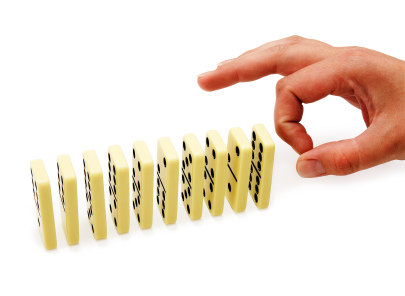
\includegraphics[height=2.1in]{event-trigger.jpg}
    \end{center}
  \end{center}
}

\begin{frame}[fragile]
  \frametitle{SQL primer \texttt{1/3}}

  \center{It always starts \textit{simple}}
  \vfill

\begin{minted}{postgresql}
create table foo(a text, b int);

select a, b
  from relation r
 where a > '2013'
\end{minted}
\end{frame}

\begin{frame}[fragile]
  \frametitle{SQL primer \texttt{2/3}}

  \center{It always starts \textit{simple enough}}
  \vfill

\begin{minted}{postgresql}
create table foo(a int, b int);

select a, b
  from relation r
 where a > '2013'
\end{minted}
\end{frame}

\begin{frame}[fragile]
  \frametitle{SQL primer \texttt{3/3}}

  \center{It always starts \textit{simple}... then we try handling \textit{time}}
  \vfill

\begin{minted}{postgresql}
create table foo(a date, b int);

select a, b
  from relation r
 where a > '2013'
\end{minted}
\end{frame}

\section{PostgreSQL Extensions}

\begin{frame}[fragile]
  \frametitle{SQL primer: Extensions}

\begin{minted}{postgresql}
create extension hstore;

create table testhstore (h hstore);

select count(*)
  from testhstore
 where h @> 'wait=>CC, public=>t';
\end{minted}
\end{frame}

\frame{
  \frametitle{PostgreSQL supports Extensions}

  \center{Data Type Specific Indexing and Query Support}
  \vfill

  \begin{itemize}
    \item Functions, Aggregates, Window Functions
    \item Data Types with Input/Output functions
    \item Casts (implicit, assignment only)
    \item Operators
    \item Operator Class, Operator Family
    \item \textit{and more...}
  \end{itemize}
}

\section{Data Modification Trigger}

\frame{
  \frametitle{Physical Model Optimisations, Business Logic}

  \center{With PostgreSQL you can tweak \texttt{INSERT}, \texttt{UPDATE}, \texttt{DELETE}}

  \vfill

  \begin{itemize}
    \item<1-> Maintain a Materialized View
    \item<1-> Apply crossing threshold discounts
    \item<2-> Trigger external actions on some events
    \item<2-> \texttt{NOTIFY} some other application parts (e.g. cache)
    \item<3-> Queue events to process later (Use \alert{PGQ})
    \item<3-> Replicate data (Slony, Londiste, Bucardo...)
  \end{itemize}
}

\begin{frame}[fragile]
  \frametitle{Data Modification Trigger Example \texttt{1/2}}

\begin{minted}{postgresql}
CREATE TABLE main_table (a int, b int);

CREATE FUNCTION trigger_func()
        RETURNS trigger
       LANGUAGE plpgsql AS '
BEGIN
  RAISE NOTICE ''trigger_func(%) called: action = %, when = %, level = %'',
               TG_ARGV[0], TG_OP, TG_WHEN, TG_LEVEL;
  RETURN NULL;
END;';
\end{minted}
\end{frame}

\begin{frame}[fragile]
  \frametitle{Data Modification Trigger Example \texttt{2/2}}

\begin{minted}{postgresql}
    CREATE TRIGGER before_ins_stmt_trig
  BEFORE INSERT ON main_table
          FOR EACH STATEMENT
 EXECUTE PROCEDURE trigger_func('before_ins_stmt');

    CREATE TRIGGER after_ins_stmt_trig
   AFTER INSERT ON main_table
          FOR EACH STATEMENT
 EXECUTE PROCEDURE trigger_func('after_ins_stmt');
\end{minted}
\end{frame}

\section{Event Triggers}

\begin{frame}[fragile]
  \frametitle{SQL \textbf{\texttt{DDL}} primer}

  \center{\textit{\textbf{D}ata \textbf{D}efinition \textbf{L}anguage}}
  \vfill

\begin{minted}{postgresql}
create table foo
 (
   id serial primary key,
   f1 text
 );

 alter table foo
  add column f2 text check (upper(f2) = f2);
\end{minted}
\end{frame}

\begin{frame}[fragile]
  \frametitle{SQL \textbf{\texttt{DDL}} primer}

  \center{Here's what \texttt{foo} looks like now}
  \vfill

\begin{minted}{postgresql}
~# \d foo
                         Table "public.foo"
 Column |  Type   |                    Modifiers                     
--------+---------+--------------------------------------------------
 id     | integer | not null default nextval('foo_id_seq'::regclass)
 f1     | text    | 
 f2     | text    | 
Indexes:
    "foo_pkey" PRIMARY KEY, btree (id)
Check constraints:
    "foo_f2_check" CHECK (upper(f2) = f2)
\end{minted}
\end{frame}

\frame{
  \frametitle{What if you could \textit{tweak} \texttt{DDL} too}

  \center{Some \textbf{DDL} Trigger use cases}
  \vfill

  \begin{itemize}
  \item Audit trail
  \item Replication Triggers
  \item Implement Local Policies
  \item Divert Execution
  \item Limited Granting of DDL privileges with \texttt{Security Definer}
    trigger functions
  \end{itemize}
}

\frame{
  \frametitle{What if you could \textit{tweak} \texttt{DDL} too}

  \center{Some \textbf{Event} Trigger use cases}
  \vfill

  \begin{itemize}
  \item<1-> \texttt{sql\_drop} (\texttt{CASCADE})
  \item<2-> Prevent Table Rewrite (except at night) (unless full moon)
  \item<3-> Create Table If Not Exists, at \texttt{INSERT} time
  \item<4-> Integrated Extension Package Management
  \end{itemize}
}

\section{Using Event Trigger}

\begin{frame}[fragile]
  \frametitle{Event Trigger Primer}

\begin{minted}{postgresql}
CREATE OR REPLACE FUNCTION abort_any_command()
  RETURNS event_trigger
 LANGUAGE plpgsql
  AS '
BEGIN
  RAISE EXCEPTION ''command % is disabled'', tg_tag;
END;
';

CREATE EVENT TRIGGER abort_ddl ON ddl_command_start
   EXECUTE PROCEDURE abort_any_command();
\end{minted}
\end{frame}

\begin{frame}[fragile]
  \frametitle{Event Trigger Primer}

  \center{Of course, the usual \texttt{ALTER} and \texttt{DROP} commands}
  \vfill

\begin{minted}{postgresql}
ALTER EVENT TRIGGER abort_ddl DISABLE;
ALTER EVENT TRIGGER abort_ddl ENABLE replica|always;
ALTER EVENT TRIGGER abort_ddl OWNER TO bob;
ALTER EVENT TRIGGER abort_ddl RENAME TO assimilated;

DROP EVENT TRIGGER abort_ddl;
\end{minted}
\end{frame}

\frame{
  \frametitle{Events}

  \center{Limited Number of Events Supported now}
  \vfill

  \begin{itemize}
    \item \texttt{ddl\_command\_start}
    \item \texttt{ddl\_command\_end}
    \item \texttt{sql\_drop} \textit{currently in review}
  \end{itemize}
}

\section{Event Trigger Tags}

\begin{frame}[fragile]
  \frametitle{Tags \texttt{1/3}}

\begin{minted}{postgresql}
~# create table bar(a int, b int);
CREATE TABLE

~# create function add1(int) returns int
   language sql as 'select \$1+1';
CREATE FUNCTION

~# drop function add1(int);
DROP FUNCTION
\end{minted}
\end{frame}

\begin{frame}[fragile]
  \frametitle{Tags \texttt{2/3}}

\begin{minted}{postgresql}
create function test_event_trigger()
        returns event_trigger as '
BEGIN
    RAISE NOTICE ''test_event_trigger: % %'', tg_event, tg_tag;
END
' language plpgsql;

create function test_event_trigger_drop_function()
        returns event_trigger as '
BEGIN
    drop function test_event_trigger() cascade;
END
' language plpgsql;

\end{minted}
\end{frame}

\begin{frame}[fragile]
  \frametitle{Tags \texttt{3/3}}

  \center{And now let's have some fun}
  \vfill

\begin{minted}{postgresql}
create event trigger drop_test_b on "ddl_command_start"
   execute procedure test_event_trigger();

create event trigger drop_test_a on "ddl_command_start"
    when tag in ('create table')
   execute procedure test_event_trigger_drop_function();

create table event_trigger_fire1 (a int);
\end{minted}
\end{frame}


\section{Event Trigger Information}

\frame{
  \frametitle{Event Triggers Information}

  \center{Currently given as magic variables available in \texttt{PLpgSQL}}
  \vfill

\begin{columns}[c]
\column{.5\textwidth} 
  \center{We have}

  \begin{itemize}
    \item \texttt{TG\_EVENT}
    \item \texttt{TG\_TAG}
      \newline
      \newline
      \newline
      \newline
  \end{itemize}

\column{.5\textwidth}
  \center{We want to add}

  \begin{itemize}
    \item \texttt{TG\_OPERATION}
    \item \texttt{TG\_OBTYPENAME}
    \item \texttt{TG\_OBJECTID}
    \item \texttt{TG\_OBJECTNAME}
    \item \texttt{TG\_SCHEMANAME}
  \end{itemize}
\end{columns}
}

\begin{frame}[fragile]
  \frametitle{What about \textit{generated} commands?}

  \center{Current proposal is \texttt{TG\_CONTEXT}. See the worked out
    tracking examples at
    \url{http://www.postgresql.org/message-id/m2han7xyzp.fsf@2ndQuadrant.fr}
  }
  \vfill

\begin{minted}{postgresql}
create event trigger track_table on ddl_command_trace
    when tag in ('create table', 'alter table', 'drop table')
 and context in ('toplevel', 'generated', 'subcommand')
execute procedure public.track_table_activity();
\end{minted}
\end{frame}

\section{Command String Normalisation}

\begin{frame}[fragile]
  \frametitle{Command String Normalisation \texttt{1/4}}

  \center{And still some more}
  \vfill

\begin{minted}{postgresql}
create schema baz
  authorization dim

  create table distributors
    (
     did  serial primary key,
     name varchar(40),
     f2   text check (upper(f2) = f2),

     unique(name) with (fillfactor=70)
    )
    with (fillfactor=70);
\end{minted}
\end{frame}

\begin{frame}[fragile]
  \frametitle{Command String Normalisation \texttt{2/4}}

\begin{minted}{postgresql}
NOTICE:  snitch event: ddl_command_end, context: GENERATED,
         tag: CREATE SEQUENCE, operation: CREATE,
        type: SEQUENCE
NOTICE:  oid: 41633, schema: baz, name: distributors_did_seq
NOTICE: command: CREATE SEQUENCE baz.distributors_did_seq;

NOTICE:  snitch event: ddl_command_end, context: SUBCOMMAND,
         tag: CREATE TABLE, operation: CREATE, type: TABLE
NOTICE:  oid: 41635, schema: baz, name: distributors
NOTICE: command: CREATE TABLE baz.distributors
 (did integer,
  name pg_catalog.varchar, 
  f2 text,
  CHECK ((upper(f2) = f2))) WITH (fillfactor=70);
\end{minted}
\end{frame}

\begin{frame}[fragile]
  \frametitle{Command String Normalisation \texttt{3/4}}

\begin{minted}{postgresql}
NOTICE:  snitch event: ddl_command_end, context: GENERATED,
         tag: CREATE INDEX, operation: CREATE, type: INDEX
NOTICE:  oid: 41643, schema: baz, name: distributors_pkey
NOTICE: command: CREATE UNIQUE INDEX distributors_pkey
                 ON baz.distributors USING btree (did);

NOTICE:  snitch event: ddl_command_end, context: GENERATED,
         tag: CREATE INDEX, operation: CREATE, type: INDEX
NOTICE:  oid: 41645, schema: baz, name: distributors_name_key
NOTICE: command: CREATE UNIQUE INDEX distributors_name_key
                 ON baz.distributors USING btree (name)
                 WITH (fillfactor=70);
\end{minted}
\end{frame}

\begin{frame}[fragile]
  \frametitle{Command String Normalisation \texttt{4/4}}

\begin{minted}{postgresql}
NOTICE:  snitch event: ddl_command_end, context: GENERATED,
         tag: ALTER SEQUENCE, operation: ALTER, type: SEQUENCE
NOTICE:  oid: 41633, schema: baz, name: distributors_did_seq
NOTICE: command: ALTER SEQUENCE baz.distributors_did_seq
                 OWNED BY baz.distributors.did;

NOTICE:  snitch event: ddl_command_end, context: TOPLEVEL,
         tag: CREATE SCHEMA, operation: CREATE, type: SCHEMA
NOTICE:  oid: 41632, schema: <NULL>, name: baz
NOTICE: command: CREATE SCHEMA baz AUTHORIZATION dim;

CREATE SCHEMA
\end{minted}
\end{frame}

\frame{
  \frametitle{\texttt{TG\_CONTEXT}}

  \center{How to get at \textit{generated} commands?}
  \newline

\begin{columns}[c]
\column{.5\textwidth} 
  \center{\alert{PRO}}
  \vfill
  \begin{itemize}
    \item consider them \texttt{DDL}s
    \item ProcessUtility()
    \item \texttt{ProcessUtilityContext}
  \end{itemize}

\column{.5\textwidth}
  \center{\alert{CONS}}
  \vfill
  \begin{itemize}
    \item the user didn't type a command
    \item clean up the code
    \item it's another kind of event
  \end{itemize}
\end{columns}
}

\section{future}

\frame{
  \frametitle{Next features}

  \center{Some features are still on the \textit{todo} list}
  \vfill

  \begin{itemize}
  \item<1-> \texttt{INSTEAD OF}
  \item<2-> \textit{table rewrite}
  \item<3-> \textit{create table on insert}
  \item<4-> \textit{add column on update}
  \end{itemize}
}

\section{Instead Of Event Triggers}

\begin{frame}[fragile]
  \frametitle{Instead Of Event Triggers \texttt{1/2}}

\begin{minted}{postgresql}
create event trigger my_create_extension
          instead of 'create extension'
   execute procedure my_create_extension();

\end{minted}
\end{frame}

\begin{frame}[fragile]
  \frametitle{Instead Of Event Triggers \texttt{2/2}}

\begin{minted}{postgresql}
create function my_create_extension()
        returns event_trigger
       language plpgsql
as '
begin
   alter event trigger my_create_extension disable;
   -- do some stuff here
   create extension tg_objectid;
   -- do some more stuff here, presumably
end;
';
\end{minted}
\end{frame}

\section{Conclusion}

\frame{
  \frametitle{Conclusion}

  \begin{center}
    Any Question? Now is the time to ask!

    \vfill

    \begin{center}
      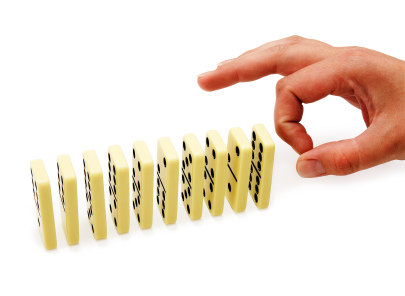
\includegraphics[height=2.1in]{event-trigger.jpg}
    \end{center}
  \end{center}
}

\end{document}
